\chapter{Excavator Setup}\label{ch:excavatorSetup}

\begin{figure}[ht]
    \centering
    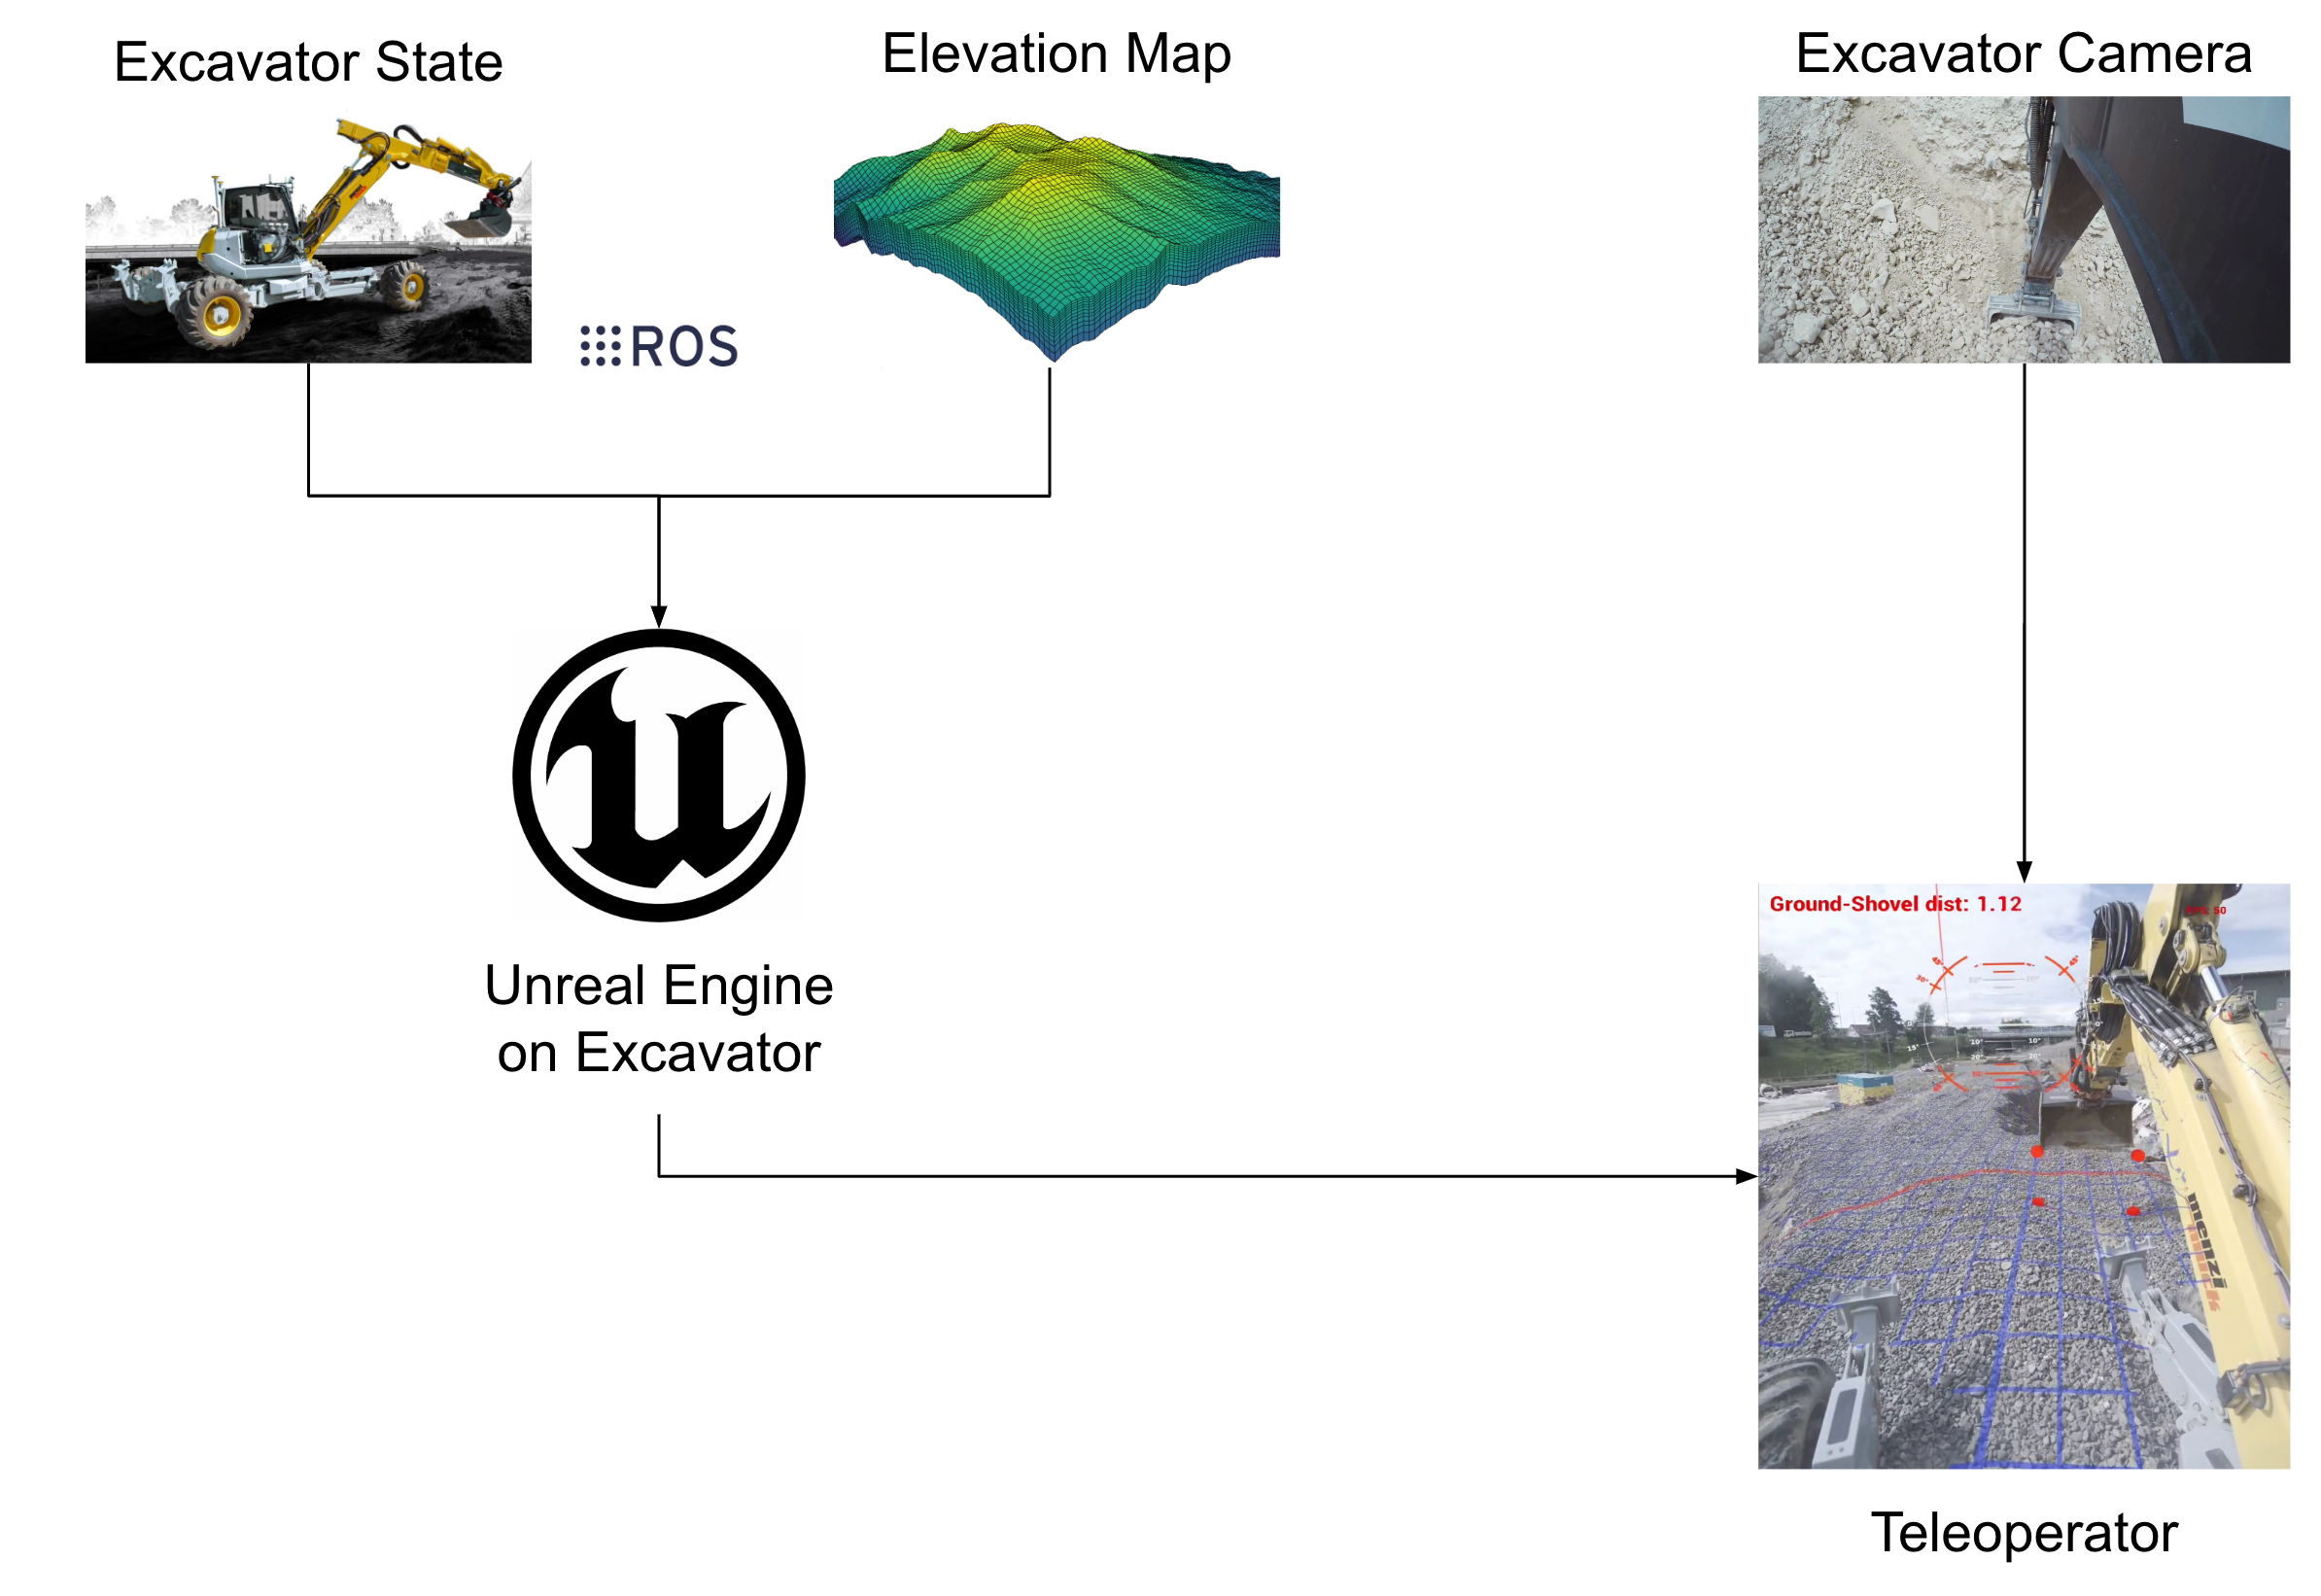
\includegraphics[scale = 0.3]{images/excavator/excavator_setup.png}
    \caption{High level excavator setup prior to this project}
    \label{fig:ex_setup}
\end{figure}

The excavator has an Unreal Engine instance running on it. In the UE instance there is a model of the excavator itself which is updated continuously using a built in ROS subscriber game component.

Another crucial input to the excavator is an elevation map which is generated from the visual input of the environment.

Through the current state of the excavator at any time it is possible to determine the parts of the camera input image which are covered by the excavator. When overlaying the elevation map onto the camera input this feature allows for the creation of a mask to cut the excavator out of the elevation map projection. This combined image input is then fed to the teleoperation setup. This is just one use case of having a real time updated simulation of the system at hand. 

In the handheld setup we can make use of this pipeline to fulfill our specific requirements and further down the road enable high level remote control inputs.
